% ===========================================================================
%  TikuOS — TikuKits DS: Priority Queue for Embedded Systems
%  Beamer Presentation
% ===========================================================================
\documentclass[aspectratio=169, 10pt]{beamer}

% ---- Theme ----------------------------------------------------------------
\usetheme{Madrid}
\usecolortheme{whale}
\setbeamertemplate{navigation symbols}{}
\setbeamertemplate{footline}{%
  \leavevmode\hbox{%
    \begin{beamercolorbox}[wd=.33\paperwidth,ht=2.5ex,dp=1ex,center]{author in head/foot}%
      \usebeamerfont{author in head/foot}\insertshortauthor
    \end{beamercolorbox}%
    \begin{beamercolorbox}[wd=.34\paperwidth,ht=2.5ex,dp=1ex,center]{title in head/foot}%
      \usebeamerfont{title in head/foot}\insertshorttitle
    \end{beamercolorbox}%
    \begin{beamercolorbox}[wd=.33\paperwidth,ht=2.5ex,dp=1ex,right]{date in head/foot}%
      \usebeamerfont{date in head/foot}\insertshortdate{}\hspace*{2em}%
      \insertframenumber{}/\inserttotalframenumber\hspace*{2ex}
    \end{beamercolorbox}}%
  \vskip0pt%
}

% ---- Packages -------------------------------------------------------------
\usepackage{listings}
\usepackage{graphicx}
\usepackage{hyperref}
\usepackage{booktabs}
\usepackage{multirow}
\usepackage{tikz}
\usetikzlibrary{arrows.meta, positioning, shapes.geometric, calc,
                decorations.pathreplacing, fit}
\usepackage{amsmath}

% ---- Code listing style ---------------------------------------------------
\lstset{
  basicstyle=\ttfamily\scriptsize,
  keywordstyle=\color{blue}\bfseries,
  commentstyle=\color{gray},
  stringstyle=\color{red!70!black},
  showstringspaces=false,
  breaklines=true,
  frame=single,
  rulecolor=\color{black!30},
  backgroundcolor=\color{blue!3},
  tabsize=4,
}
\lstdefinestyle{cstyle}{
  language=C,
  morekeywords={uint8_t,uint16_t,uint32_t,int32_t,
                tiku_kits_ds_elem_t,
                TIKU_KITS_DS_OK,TIKU_KITS_DS_ERR_NULL,
                TIKU_KITS_DS_ERR_FULL,TIKU_KITS_DS_ERR_EMPTY,
                TIKU_KITS_DS_ERR_PARAM,
                TIKU_KITS_DS_PQUEUE_MAX_LEVELS,
                TIKU_KITS_DS_PQUEUE_MAX_PER_LEVEL,
                NULL},
}

% ---- Metadata -------------------------------------------------------------
\title[TikuKits DS]{TikuKits DS: Priority Queue for Embedded Systems}
\subtitle{Simple. Ubiquitous. Intelligence, Everywhere.}
\author[Ambuj Varshney]{Ambuj Varshney \\ \texttt{ambuj@tiku-os.org}}
\date{\today}

% ===========================================================================
\begin{document}

% ---------------------------------------------------------------------------
\begin{frame}
\titlepage
\end{frame}

% ---------------------------------------------------------------------------
\begin{frame}{Outline}
\tableofcontents
\end{frame}

% ===========================================================================
\section{Motivation}
% ===========================================================================

\begin{frame}{Why a Priority Queue on MCUs?}
\begin{columns}[T]
\begin{column}{0.48\textwidth}
\begin{block}{Embedded Use Cases}
\begin{itemize}
  \item \textbf{Event dispatch} --- critical vs.\ normal vs.\ low-priority events
  \item \textbf{Task scheduling} --- urgent sensor reads before background logging
  \item \textbf{Alarm levels} --- emergency alarms processed before informational
  \item \textbf{Message routing} --- prioritize control messages over telemetry
\end{itemize}
\end{block}

\begin{block}{Constraints}
\begin{itemize}
  \item No heap allocation
  \item Limited RAM (2--8\,KB)
  \item Deterministic $O(L)$ dequeue, $L$ = number of levels
  \item Must be interrupt-safe with bounded time
\end{itemize}
\end{block}
\end{column}

\begin{column}{0.48\textwidth}
\begin{center}
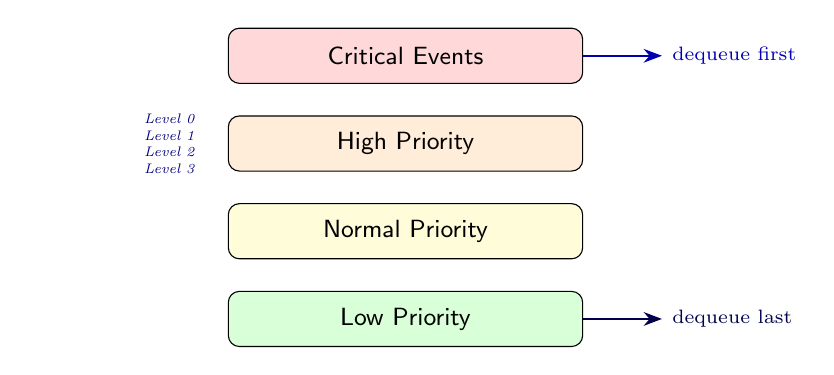
\begin{tikzpicture}[
    >=Stealth, node distance=0.5cm
  ]
  \node[draw, rounded corners, minimum height=0.7cm,
        text centered, font=\small\sffamily, fill=red!15,
        minimum width=4.5cm] (crit) {Critical Events};
  \node[draw, rounded corners, minimum height=0.7cm,
        text centered, font=\small\sffamily, fill=orange!15,
        minimum width=4.5cm, below=0.4cm of crit] (high)
    {High Priority};
  \node[draw, rounded corners, minimum height=0.7cm,
        text centered, font=\small\sffamily, fill=yellow!15,
        minimum width=4.5cm, below=0.4cm of high] (norm)
    {Normal Priority};
  \node[draw, rounded corners, minimum height=0.7cm,
        text centered, font=\small\sffamily, fill=green!15,
        minimum width=4.5cm, below=0.4cm of norm] (low)
    {Low Priority};
  \draw[->, thick, blue!70!black] (crit.east) -- ++(1.0,0)
    node[right, font=\scriptsize] {dequeue first};
  \draw[->, thick, blue!30!black] (low.east) -- ++(1.0,0)
    node[right, font=\scriptsize] {dequeue last};

  \node[left=0.3cm of high, font=\tiny\itshape, text=blue!50!black,
        text width=2cm, align=right] {Level 0\\Level 1\\Level 2\\Level 3};
\end{tikzpicture}
\end{center}

\vspace{0.5em}
\begin{alertblock}{Design Goal}
Array of mini ring buffers --- \textbf{NOT} a heap-based priority queue.
Simple, deterministic, and perfect for 3--4 priority levels.
\end{alertblock}
\end{column}
\end{columns}
\end{frame}

% ===========================================================================
\section{Architecture}
% ===========================================================================

\begin{frame}{How It Works: Array of Ring Buffers}
\begin{columns}[T]
\begin{column}{0.48\textwidth}
\textbf{Key insight:} For a small number of priority levels (3--4),
a heap is overkill. Instead, maintain one FIFO ring buffer per level.

\vspace{0.5em}
\textbf{Enqueue:} Insert into the ring buffer at the given priority level --- $O(1)$.

\vspace{0.5em}
\textbf{Dequeue:} Scan from level 0 (highest priority) upward, return
the first non-empty level's head element --- $O(L)$ where $L \leq 4$.

\vspace{0.5em}
\textbf{FIFO within level:} Items at the same priority are served
in insertion order (first-in, first-out).

\vspace{0.5em}
\begin{block}{Complexity}
\begin{tabular}{@{}ll@{}}
Enqueue: & $O(1)$ \\
Dequeue: & $O(L)$, $L \leq 4$ \\
Peek:    & $O(L)$ \\
Size:    & $O(L)$ \\
\end{tabular}
\end{block}
\end{column}

\begin{column}{0.48\textwidth}
\begin{center}
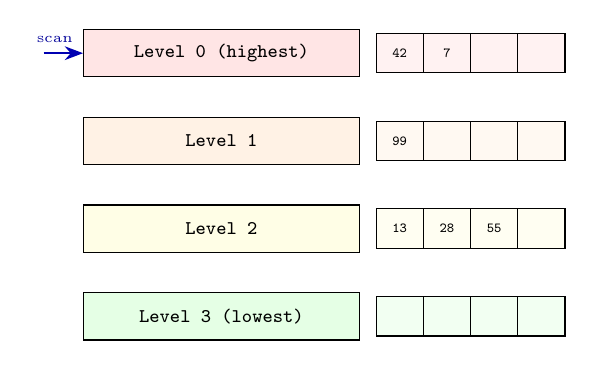
\begin{tikzpicture}[
    >=Stealth,
    level/.style={draw, minimum width=3.5cm, minimum height=0.6cm,
                  font=\scriptsize\ttfamily},
    cell/.style={draw, minimum width=0.6cm, minimum height=0.5cm,
                 font=\tiny\ttfamily}
  ]
  % Level 0
  \node[level, fill=red!10] (l0) {Level 0 (highest)};
  \foreach \x/\v in {0/42, 1/7, 2/{}, 3/{}} {
    \node[cell, fill=red!5, right=\x*0.6cm of l0.east, anchor=west,
          xshift=0.2cm] (c0\x) {\v};
  }

  % Level 1
  \node[level, fill=orange!10, below=0.5cm of l0] (l1) {Level 1};
  \foreach \x/\v in {0/99, 1/{}, 2/{}, 3/{}} {
    \node[cell, fill=orange!5, right=\x*0.6cm of l1.east, anchor=west,
          xshift=0.2cm] (c1\x) {\v};
  }

  % Level 2
  \node[level, fill=yellow!10, below=0.5cm of l1] (l2) {Level 2};
  \foreach \x/\v in {0/13, 1/28, 2/55, 3/{}} {
    \node[cell, fill=yellow!5, right=\x*0.6cm of l2.east, anchor=west,
          xshift=0.2cm] (c2\x) {\v};
  }

  % Level 3
  \node[level, fill=green!10, below=0.5cm of l2] (l3) {Level 3 (lowest)};
  \foreach \x/\v in {0/{}, 1/{}, 2/{}, 3/{}} {
    \node[cell, fill=green!5, right=\x*0.6cm of l3.east, anchor=west,
          xshift=0.2cm] (c3\x) {\v};
  }

  % Dequeue arrow
  \draw[->, thick, blue!70!black] ([xshift=-0.5cm]l0.west) -- (l0.west)
    node[above left, font=\tiny, text=blue!60!black] {scan};
\end{tikzpicture}
\end{center}
\end{column}
\end{columns}
\end{frame}

% ===========================================================================
\section{Data Structure}
% ===========================================================================

\begin{frame}[fragile]{The \texttt{tiku\_kits\_ds\_pqueue} Structures}
\begin{columns}[T]
\begin{column}{0.48\textwidth}
\begin{lstlisting}[style=cstyle,
  title={ds/pqueue/tiku\_kits\_ds\_pqueue.h}]
struct tiku_kits_ds_pqueue_level {
    tiku_kits_ds_elem_t data[
        TIKU_KITS_DS_PQUEUE_MAX_PER_LEVEL];
    uint8_t head;     /* next to dequeue */
    uint8_t tail;     /* next free slot  */
    uint8_t count;    /* elements here   */
    uint8_t capacity; /* runtime cap     */
};

struct tiku_kits_ds_pqueue {
    struct tiku_kits_ds_pqueue_level
        levels[TIKU_KITS_DS_PQUEUE_MAX_LEVELS];
    uint8_t n_levels;
};
\end{lstlisting}
\end{column}

\begin{column}{0.48\textwidth}
\textbf{Memory footprint} (default config):\\
Per level: $8 \times 4 + 4 = 36$ bytes\\
Total: $4 \times 36 + 1 = 145$ bytes\\
All statically allocated --- no heap.

\vspace{0.5em}
\begin{block}{Ring Buffer Per Level}
Each level is a circular buffer with \texttt{head}, \texttt{tail}, and \texttt{count}.
Wrap-around uses modulo: \texttt{tail = (tail + 1) \% capacity}.
\end{block}

\vspace{0.5em}
\begin{alertblock}{Not a Heap}
No parent/child relationships, no sift-up/down.
Just an array of independent FIFO queues indexed by priority.
\end{alertblock}
\end{column}
\end{columns}
\end{frame}

% ===========================================================================
\section{API Reference}
% ===========================================================================

\begin{frame}[fragile]{Complete API}
\begin{table}
\centering
\small
\begin{tabular}{@{}lp{8cm}@{}}
\toprule
\textbf{Function} & \textbf{Description} \\
\midrule
\texttt{tiku\_kits\_ds\_pqueue\_init(pq, n, per)}
  & Initialize with \texttt{n} priority levels, \texttt{per} slots each \\
\midrule
\texttt{tiku\_kits\_ds\_pqueue\_enqueue(pq, val, pri)}
  & Insert \texttt{val} at priority level \texttt{pri} (0 = highest) \\
\texttt{tiku\_kits\_ds\_pqueue\_dequeue(pq, \&val)}
  & Remove highest-priority element (scans level 0 first) \\
\texttt{tiku\_kits\_ds\_pqueue\_peek(pq, \&val)}
  & Read highest-priority element without removing \\
\midrule
\texttt{tiku\_kits\_ds\_pqueue\_clear(pq)}
  & Reset all levels to empty \\
\texttt{tiku\_kits\_ds\_pqueue\_size(pq)}
  & Total element count across all levels \\
\texttt{tiku\_kits\_ds\_pqueue\_empty(pq)}
  & Returns 1 if all levels are empty \\
\bottomrule
\end{tabular}
\end{table}

\vspace{0.3em}
\begin{alertblock}{Priority Convention}
Level 0 is \textbf{highest} priority. Dequeue always returns from the
lowest-numbered non-empty level. Within a level, elements are served FIFO.
\end{alertblock}
\end{frame}

% ===========================================================================
\section{Configuration}
% ===========================================================================

\begin{frame}[fragile]{Compile-Time Configuration}
\begin{columns}[T]
\begin{column}{0.48\textwidth}
\begin{lstlisting}[style=cstyle,
  title={Configurable parameters}]
/* Maximum priority levels */
#ifndef TIKU_KITS_DS_PQUEUE_MAX_LEVELS
#define TIKU_KITS_DS_PQUEUE_MAX_LEVELS 4
#endif

/* Max elements per level */
#ifndef TIKU_KITS_DS_PQUEUE_MAX_PER_LEVEL
#define TIKU_KITS_DS_PQUEUE_MAX_PER_LEVEL 8
#endif
\end{lstlisting}

\vspace{0.3em}
\begin{block}{Shared Return Codes}
Defined in \texttt{tiku\_kits\_ds.h}:
\begin{itemize}
  \item \texttt{TIKU\_KITS\_DS\_OK} (0)
  \item \texttt{TIKU\_KITS\_DS\_ERR\_NULL} ($-1$)
  \item \texttt{TIKU\_KITS\_DS\_ERR\_FULL} ($-2$)
  \item \texttt{TIKU\_KITS\_DS\_ERR\_EMPTY} ($-3$)
  \item \texttt{TIKU\_KITS\_DS\_ERR\_PARAM} ($-4$)
\end{itemize}
\end{block}
\end{column}

\begin{column}{0.48\textwidth}
\begin{lstlisting}[style=cstyle,
  title={Runtime initialization}]
struct tiku_kits_ds_pqueue pq;

/* 3 levels, 4 slots each */
tiku_kits_ds_pqueue_init(&pq, 3, 4);

/* Or customize at compile time: */
/* -DTIKU_KITS_DS_PQUEUE_MAX_LEVELS=8
 * -DTIKU_KITS_DS_PQUEUE_MAX_PER_LEVEL=16
 */
\end{lstlisting}

\vspace{0.3em}
\begin{table}
\centering
\scriptsize
\begin{tabular}{@{}rrr@{}}
\toprule
\textbf{Levels} & \textbf{Per Level} & \textbf{RAM (bytes)} \\
\midrule
2 & 4  & $\sim$73 \\
3 & 4  & $\sim$109 \\
4 & 8  & $\sim$145 \\
4 & 16 & $\sim$273 \\
\bottomrule
\end{tabular}
\end{table}
\end{column}
\end{columns}
\end{frame}

% ===========================================================================
\section{Implementation Details}
% ===========================================================================

\begin{frame}[fragile]{Enqueue: Insert at Priority Level}
\begin{lstlisting}[style=cstyle,
  title={tiku\_kits\_ds\_pqueue.c --- enqueue}]
int tiku_kits_ds_pqueue_enqueue(struct tiku_kits_ds_pqueue *pq,
                                tiku_kits_ds_elem_t value,
                                uint8_t priority)
{
    struct tiku_kits_ds_pqueue_level *lvl;

    if (pq == NULL) {
        return TIKU_KITS_DS_ERR_NULL;
    }
    if (priority >= pq->n_levels) {
        return TIKU_KITS_DS_ERR_PARAM;
    }

    lvl = &pq->levels[priority];

    if (lvl->count >= lvl->capacity) {
        return TIKU_KITS_DS_ERR_FULL;
    }

    lvl->data[lvl->tail] = value;
    lvl->tail = (lvl->tail + 1) % lvl->capacity;
    lvl->count++;
    return TIKU_KITS_DS_OK;
}
\end{lstlisting}

\begin{block}{$O(1)$ Insertion}
Direct array index to the priority level. Ring buffer tail-insert with modular wrap.
No shifting, no rebalancing, no comparisons.
\end{block}
\end{frame}

% ---------------------------------------------------------------------------
\begin{frame}[fragile]{Dequeue: Scan from Highest Priority}
\begin{lstlisting}[style=cstyle,
  title={tiku\_kits\_ds\_pqueue.c --- dequeue}]
int tiku_kits_ds_pqueue_dequeue(struct tiku_kits_ds_pqueue *pq,
                                tiku_kits_ds_elem_t *value)
{
    uint8_t i;
    struct tiku_kits_ds_pqueue_level *lvl;

    if (pq == NULL || value == NULL) {
        return TIKU_KITS_DS_ERR_NULL;
    }

    /* Scan from highest priority (level 0) to lowest */
    for (i = 0; i < pq->n_levels; i++) {
        lvl = &pq->levels[i];
        if (lvl->count > 0) {
            *value = lvl->data[lvl->head];
            lvl->head = (lvl->head + 1) % lvl->capacity;
            lvl->count--;
            return TIKU_KITS_DS_OK;
        }
    }

    return TIKU_KITS_DS_ERR_EMPTY;
}
\end{lstlisting}

\begin{block}{$O(L)$ Dequeue}
Linear scan over at most $L$ levels (typically 3--4). First non-empty level
wins. FIFO order within that level via ring buffer head-pop.
\end{block}
\end{frame}

% ===========================================================================
\section{Examples}
% ===========================================================================

\begin{frame}[fragile]{Example 1: Event Dispatch System}
\begin{lstlisting}[style=cstyle,
  title={Event dispatcher with 4 priority levels}]
struct tiku_kits_ds_pqueue event_q;
tiku_kits_ds_elem_t event_id;

/* 4 levels: CRITICAL=0, HIGH=1, NORMAL=2, LOW=3 */
tiku_kits_ds_pqueue_init(&event_q, 4, 8);

/* ISR posts critical alarm */
tiku_kits_ds_pqueue_enqueue(&event_q, EVT_OVERTEMP, 0);

/* Background task posts telemetry event */
tiku_kits_ds_pqueue_enqueue(&event_q, EVT_LOG_DATA, 3);

/* Timer posts periodic sensor read */
tiku_kits_ds_pqueue_enqueue(&event_q, EVT_SENSOR_READ, 2);

/* Main loop processes events in priority order */
while (!tiku_kits_ds_pqueue_empty(&event_q)) {
    tiku_kits_ds_pqueue_dequeue(&event_q, &event_id);
    dispatch_event(event_id);
    /* Order: EVT_OVERTEMP, EVT_SENSOR_READ, EVT_LOG_DATA */
}
\end{lstlisting}
\end{frame}

% ---------------------------------------------------------------------------
\begin{frame}[fragile]{Example 2: Task Scheduler with Peek}
\begin{columns}[T]
\begin{column}{0.52\textwidth}
\begin{lstlisting}[style=cstyle,
  title={Task scheduler with priority levels}]
struct tiku_kits_ds_pqueue tasks;
tiku_kits_ds_elem_t task_id;

/* 3 levels: URGENT=0, NORMAL=1, IDLE=2 */
tiku_kits_ds_pqueue_init(&tasks, 3, 4);

/* Enqueue tasks */
tiku_kits_ds_pqueue_enqueue(
    &tasks, TASK_WATCHDOG, 0);
tiku_kits_ds_pqueue_enqueue(
    &tasks, TASK_SENSOR, 1);
tiku_kits_ds_pqueue_enqueue(
    &tasks, TASK_DISPLAY, 1);
tiku_kits_ds_pqueue_enqueue(
    &tasks, TASK_SLEEP, 2);

/* Peek without removing */
tiku_kits_ds_pqueue_peek(&tasks, &task_id);
/* task_id == TASK_WATCHDOG */

/* Process all tasks */
while (tiku_kits_ds_pqueue_dequeue(
       &tasks, &task_id) ==
       TIKU_KITS_DS_OK) {
    run_task(task_id);
}
\end{lstlisting}
\end{column}

\begin{column}{0.44\textwidth}
\begin{center}
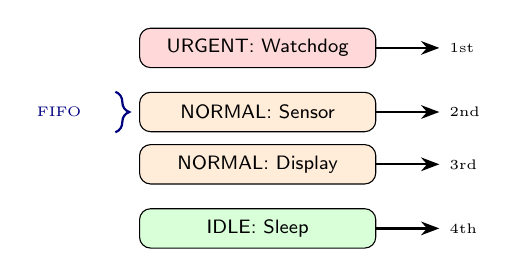
\begin{tikzpicture}[
    >=Stealth,
    box/.style={draw, rounded corners, minimum width=3cm,
                minimum height=0.5cm, font=\scriptsize\sffamily}
  ]
  \node[box, fill=red!15] (u) {URGENT: Watchdog};
  \node[box, fill=orange!15, below=0.3cm of u] (n1) {NORMAL: Sensor};
  \node[box, fill=orange!15, below=0.15cm of n1] (n2) {NORMAL: Display};
  \node[box, fill=green!15, below=0.3cm of n2] (i) {IDLE: Sleep};

  \draw[->, thick] (u.east) -- ++(0.8,0) node[right, font=\tiny] {1st};
  \draw[->, thick] (n1.east) -- ++(0.8,0) node[right, font=\tiny] {2nd};
  \draw[->, thick] (n2.east) -- ++(0.8,0) node[right, font=\tiny] {3rd};
  \draw[->, thick] (i.east) -- ++(0.8,0) node[right, font=\tiny] {4th};

  \draw[decorate, decoration={brace, amplitude=5pt, mirror},
        thick, blue!50!black]
    ([xshift=-0.3cm]n1.south west) -- ([xshift=-0.3cm]n1.north west)
    node[midway, left=0.3cm, font=\tiny, text=blue!50!black] {FIFO};
\end{tikzpicture}
\end{center}

\vspace{0.5em}
\begin{block}{FIFO Within Level}
Tasks at the same priority level are processed
in the order they were enqueued. Watchdog (urgent)
always runs first regardless of insertion order.
\end{block}
\end{column}
\end{columns}
\end{frame}

% ---------------------------------------------------------------------------
\begin{frame}[fragile]{Example 3: Alarm Level System}
\begin{lstlisting}[style=cstyle,
  title={Multi-level alarm processing}]
#define ALARM_EMERGENCY  0  /* system shutdown imminent */
#define ALARM_WARNING    1  /* operator attention needed */
#define ALARM_INFO       2  /* logged but no action */

struct tiku_kits_ds_pqueue alarms;
tiku_kits_ds_elem_t alarm_code;

tiku_kits_ds_pqueue_init(&alarms, 3, 4);

/* Sensor ISR posts alarms at different levels */
tiku_kits_ds_pqueue_enqueue(&alarms, 0x01, ALARM_INFO);
tiku_kits_ds_pqueue_enqueue(&alarms, 0x10, ALARM_EMERGENCY);
tiku_kits_ds_pqueue_enqueue(&alarms, 0x05, ALARM_WARNING);

/* Emergency alarm always processed first */
tiku_kits_ds_pqueue_dequeue(&alarms, &alarm_code);
/* alarm_code == 0x10 (emergency) */

/* Clear all pending alarms after system reset */
tiku_kits_ds_pqueue_clear(&alarms);
\end{lstlisting}
\end{frame}

% ===========================================================================
\section{Ring Buffer Internals}
% ===========================================================================

\begin{frame}{Ring Buffer Mechanics Per Level}
\begin{columns}[T]
\begin{column}{0.48\textwidth}
\begin{center}
\textbf{Enqueue Operation}
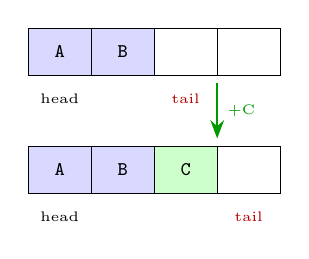
\begin{tikzpicture}[
    cell/.style={draw, minimum width=0.8cm, minimum height=0.6cm,
                 font=\scriptsize\ttfamily},
    >=Stealth
  ]
  \foreach \x/\v/\c in {0/A/blue!15, 1/B/blue!15, 2/{}/white, 3/{}/white} {
    \node[cell, fill=\c] (e\x) at (\x*0.8, 0) {\v};
  }
  \node[font=\tiny, below=0.1cm of e0] {head};
  \node[font=\tiny, below=0.1cm of e2, text=red!70!black] {tail};

  % After enqueue C
  \foreach \x/\v/\c in {0/A/blue!15, 1/B/blue!15, 2/C/green!20, 3/{}/white} {
    \node[cell, fill=\c] (f\x) at (\x*0.8, -1.5) {\v};
  }
  \node[font=\tiny, below=0.1cm of f0] {head};
  \node[font=\tiny, below=0.1cm of f3, text=red!70!black] {tail};

  \draw[->, thick, green!60!black] (2.0, -0.4) -- (2.0, -1.1)
    node[midway, right, font=\tiny] {+C};
\end{tikzpicture}
\end{center}

\vspace{0.5em}
\texttt{data[tail] = value;}\\
\texttt{tail = (tail + 1) \% capacity;}\\
\texttt{count++;}
\end{column}

\begin{column}{0.48\textwidth}
\begin{center}
\textbf{Dequeue Operation}
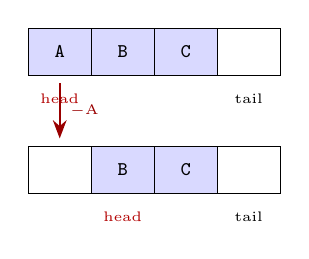
\begin{tikzpicture}[
    cell/.style={draw, minimum width=0.8cm, minimum height=0.6cm,
                 font=\scriptsize\ttfamily},
    >=Stealth
  ]
  \foreach \x/\v/\c in {0/A/blue!15, 1/B/blue!15, 2/C/blue!15, 3/{}/white} {
    \node[cell, fill=\c] (e\x) at (\x*0.8, 0) {\v};
  }
  \node[font=\tiny, below=0.1cm of e0, text=red!70!black] {head};
  \node[font=\tiny, below=0.1cm of e3] {tail};

  % After dequeue A
  \foreach \x/\v/\c in {0/{}/white, 1/B/blue!15, 2/C/blue!15, 3/{}/white} {
    \node[cell, fill=\c] (f\x) at (\x*0.8, -1.5) {\v};
  }
  \node[font=\tiny, below=0.1cm of f1, text=red!70!black] {head};
  \node[font=\tiny, below=0.1cm of f3] {tail};

  \draw[->, thick, red!60!black] (0.0, -0.4) -- (0.0, -1.1)
    node[midway, right, font=\tiny] {$-$A};
\end{tikzpicture}
\end{center}

\vspace{0.5em}
\texttt{*value = data[head];}\\
\texttt{head = (head + 1) \% capacity;}\\
\texttt{count-{}-;}
\end{column}
\end{columns}

\vspace{0.5em}
\begin{block}{Wrap-Around}
When \texttt{tail} reaches the end of the array, it wraps to index 0
via modulo arithmetic. This allows continuous enqueue/dequeue without
shifting elements --- $O(1)$ for both operations.
\end{block}
\end{frame}

% ===========================================================================
\section{Heap vs.\ Array-of-Queues}
% ===========================================================================

\begin{frame}{Why Not a Binary Heap?}
\begin{columns}[T]
\begin{column}{0.48\textwidth}
\begin{block}{Binary Heap}
\begin{itemize}
  \item $O(\log n)$ enqueue and dequeue
  \item Good for hundreds/thousands of priorities
  \item Complex sift-up/sift-down logic
  \item No FIFO guarantee within same priority
  \item Higher code size
\end{itemize}
\end{block}
\end{column}

\begin{column}{0.48\textwidth}
\begin{block}{Array of Ring Buffers (ours)}
\begin{itemize}
  \item $O(1)$ enqueue, $O(L)$ dequeue ($L \leq 4$)
  \item Perfect for 2--4 discrete priority levels
  \item Trivial implementation ($\sim$60 lines of C)
  \item FIFO within each priority level
  \item Minimal code and RAM footprint
\end{itemize}
\end{block}
\end{column}
\end{columns}

\vspace{0.5em}
\begin{table}
\centering
\small
\begin{tabular}{@{}lccc@{}}
\toprule
& \textbf{Heap} & \textbf{Array-of-Queues} & \textbf{Winner} \\
\midrule
Enqueue     & $O(\log n)$  & $O(1)$    & Array \\
Dequeue     & $O(\log n)$  & $O(L)$    & Array ($L\leq4$) \\
FIFO order  & No           & Yes       & Array \\
Code size   & $\sim$200 LOC & $\sim$60 LOC & Array \\
Best for    & Many levels  & Few levels & Depends \\
\bottomrule
\end{tabular}
\end{table}
\end{frame}

% ===========================================================================
\section{Test Suite}
% ===========================================================================

\begin{frame}{Test Cases Overview}
\begin{table}
\centering
\small
\begin{tabular}{@{}clp{7cm}@{}}
\toprule
\textbf{\#} & \textbf{Test Function} & \textbf{What It Verifies} \\
\midrule
1 & \texttt{test\_kits\_ds\_pqueue\_init}
  & Proper initialization, parameter validation \\
2 & \texttt{test\_kits\_ds\_pqueue\_basic\_priority}
  & High-priority dequeued before low-priority \\
3 & \texttt{test\_kits\_ds\_pqueue\_multi\_level}
  & Correct ordering across all 4 levels \\
4 & \texttt{test\_kits\_ds\_pqueue\_dequeue\_order}
  & FIFO order within the same priority level \\
5 & \texttt{test\_kits\_ds\_pqueue\_peek}
  & Peek returns highest-priority without removing \\
6 & \texttt{test\_kits\_ds\_pqueue\_full\_level}
  & ERR\_FULL when a level is at capacity \\
7 & \texttt{test\_kits\_ds\_pqueue\_empty\_check}
  & Empty detection and ERR\_EMPTY on dequeue \\
8 & \texttt{test\_kits\_ds\_pqueue\_clear\_reset}
  & Clear resets all levels, queue reusable \\
9 & \texttt{test\_kits\_ds\_pqueue\_null\_inputs}
  & All functions reject NULL with ERR\_NULL \\
\bottomrule
\end{tabular}
\end{table}
\end{frame}

% ===========================================================================
\section{Summary}
% ===========================================================================

\begin{frame}{Summary}
\begin{columns}[T]
\begin{column}{0.48\textwidth}
\begin{block}{What We Built}
\begin{itemize}
  \item Multi-level priority queue
  \item Array of FIFO ring buffers (not a heap)
  \item $O(1)$ enqueue, $O(L)$ dequeue
  \item FIFO ordering within each priority level
  \item 145 bytes RAM (default config), no heap
\end{itemize}
\end{block}

\begin{block}{Key Design Choices}
\begin{itemize}
  \item Level 0 = highest priority
  \item Ring buffer per level avoids shifting
  \item Modulo wrap for circular indexing
  \item Separate capacity per level at runtime
\end{itemize}
\end{block}
\end{column}

\begin{column}{0.48\textwidth}
\begin{block}{Use Cases}
\begin{itemize}
  \item Event dispatch (critical/high/normal/low)
  \item Task scheduling with urgency levels
  \item Multi-level alarm processing
  \item Message routing by importance
\end{itemize}
\end{block}

\begin{block}{Files}
\scriptsize
\begin{tabular}{@{}lp{4.5cm}@{}}
Header: & \texttt{ds/pqueue/tiku\_kits\_ds\_pqueue.h} \\
Source: & \texttt{ds/pqueue/tiku\_kits\_ds\_pqueue.c} \\
Tests: & \texttt{tests/ds/test\_kits\_ds\_pqueue.c} \\
Common: & \texttt{ds/tiku\_kits\_ds.h} \\
\end{tabular}
\end{block}
\end{column}
\end{columns}
\end{frame}

% ---------------------------------------------------------------------------
\begin{frame}{Thank You}
\begin{center}
\Large\textbf{TikuKits DS: Priority Queue}\\[0.5em]
\normalsize Deterministic Priority Dispatch for Physical AI Endpoints\\[1.5em]

\begin{tabular}{rl}
  Repository: & \url{https://github.com/tikuos/tikuOS} \\
  License:    & Apache 2.0 \\
  Common:     & \texttt{tikukits/ds/tiku\_kits\_ds.h} \\
  Header:     & \texttt{tikukits/ds/pqueue/tiku\_kits\_ds\_pqueue.h} \\
  Source:     & \texttt{tikukits/ds/pqueue/tiku\_kits\_ds\_pqueue.c} \\
  Tests:      & \texttt{tikukits/tests/ds/test\_kits\_ds\_pqueue.c} \\
\end{tabular}
\end{center}
\end{frame}

\end{document}
